\begin{quote}
This is part 31 of Categories for Programmers. Previously:
\href{https://bartoszmilewski.com/2017/08/26/lawvere-theories/}{Lawvere
Theories}. See the
\href{https://bartoszmilewski.com/2014/10/28/category-theory-for-programmers-the-preface/}{Table
of Contents}\href{https://bartoszmilewski.com/2017/07/22/topoi/}{.}
\end{quote}

There is no good place to end a book on category theory. There's always
more to learn. Category theory is a vast subject. At the same time, it's
obvious that the same themes, concepts, and patterns keep showing up
over and over again. There is a saying that all concepts are Kan
extensions and, indeed, you can use Kan extensions to derive limits,
colimits, adjunctions, monads, the Yoneda lemma, and much more. The
notion of a category itself arises at all levels of abstraction, and so
does the concept of a monoid and a monad. Which one is the most basic?
As it turns out they are all interrelated, one leading to another in a
never-ending cycle of abstractions. I decided that showing these
interconnections might be a good way to end this book.

\section{Bicategories}\label{bicategories}

One of the most difficult aspects of category theory is the constant
switching of perspectives. Take the category of sets, for instance. We
are used to defining sets in terms of elements. An empty set has no
elements. A singleton set has one element. A cartesian product of two
sets is a set of pairs, and so on. But when talking about the category
\textbf{Set} I asked you to forget about the contents of sets and
instead concentrate on morphisms (arrows) between them. You were
allowed, from time to time, to peek under the covers to see what a
particular universal construction in \textbf{Set} described in terms of
elements. The terminal object turned out to be a set with one element,
and so on. But these were just sanity checks.

A functor is defined as a mapping of categories. It's natural to
consider a mapping as a morphism in a category. A functor turned out to
be a morphism in the category of categories (small categories, if we
want to avoid questions about size). By treating a functor as an arrow,
we forfeit the information about its action on the internals of a
category (its objects and morphisms), just like we forfeit the
information about the action of a function on elements of a set when we
treat it as an arrow in \textbf{Set}. But functors between any two
categories also form a category. This time you are asked to consider
something that was an arrow in one category to be an object in another.
In a functor category functors are objects and natural transformations
are morphisms. We have discovered that the same thing can be an arrow in
one category and an object in another. The naive view of objects as
nouns and arrows as verbs doesn't hold.

Instead of switching between two views, we can try to merge them into
one. This is how we get the concept of a 2-category, in which objects
are called 0-cells, morphisms are 1-cells, and morphisms between
morphisms are 2-cells.

\hypertarget{attachment_9117}{}
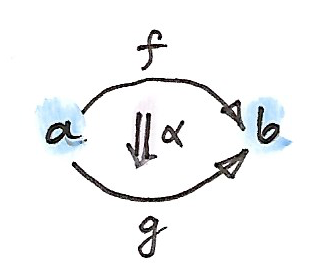
\includegraphics[width=1.53125in]{images/twocat.png}

0-cells a, b; 1-cells f, g; and a 2-cell α.

The category of categories \textbf{Cat} is an immediate example. We have
categories as 0-cells, functors as 1-cells, and natural transformations
as 2-cells. The laws of a 2-category tell us that 1-cells between any
two 0-cells form a category (in other words, \code{C(a,\ b)} is a
hom-category rather than a hom-set). This fits nicely with our earlier
assertion that functors between any two categories form a functor
category.

In particular, 1-cells from any 0-cell back to itself also form a
category, the hom-category \code{C(a,\ a)}; but that category has even
more structure. Members of \code{C(a,\ a)} can be viewed as arrows in
\textbf{C} or as objects in \code{C(a,\ a)}. As arrows, they can be
composed with each other. But when we look at them as objects, the
composition becomes a mapping from a pair of objects to an object. In
fact it looks very much like a product --- a tensor product to be
precise. This tensor product has a unit: the identity 1-cell. It turns
out that, in any 2-category, a hom-category \code{C(a,\ a)} is
automatically a monoidal category with the tensor product defined as
composition of 1-cells. Associativity and unit laws simply fall out from
the corresponding category laws.

Let's see what this means in our canonical example of a 2-category
\textbf{Cat}. The hom-category \code{Cat(a,\ a)} is the category of
endofunctors on \code{a}. Endofunctor composition plays the role of a
tensor product in it. The identity functor is the unit with respect to
this product. We've seen before that endofunctors form a monoidal
category (we used this fact in the definition of a monad), but now we
see that this is a more general phenomenon: endo-1-cells in any
2-category form a monoidal category. We'll come back to it later when we
generalize monads.

You might recall that, in a general monoidal category, we did not insist
on the monoid laws being satisfied on the nose. It was often enough for
the unit laws and the associativity laws to be satisfied up to
isomorphism. In a 2-category, monoidal laws in \code{C(a,\ a)} follow
from composition laws for 1-cells. These laws are strict, so we will
always get a strict monoidal category. It is, however, possible to relax
these laws as well. We can say, for instance, that a composition of the
identity 1-cell \code{ida} with another 1-cell,
\code{f\ ::\ a\ ->\ b}, is isomorphic, rather than equal,
to \code{f}. Isomorphism of 1-cells is defined using 2-cells. In other
words, there is a 2-cell:

\begin{verbatim}
ρ :: f ∘ ida -> f
\end{verbatim}

that has an inverse.

\hypertarget{attachment_9107}{}
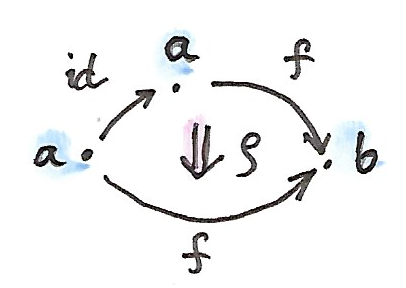
\includegraphics[width=1.70833in]{images/bicat.png}

Identity law in a bicategory holds up to isomorphism (an invertible
2-cell ρ).

We can do the same for the left identity and associativity laws. This
kind of relaxed 2-category is called a bicategory (there are some
additional coherency laws, which I will omit here).

As expected, endo-1-cells in a bicategory form a general monoidal
category with non-strict laws.

An interesting example of a bicategory is the category of spans. A span
between two objects \code{a} and \code{b} is an object \code{x}
and a pair of morphisms:

\begin{verbatim}
f :: x -> a g :: x -> b
\end{verbatim}

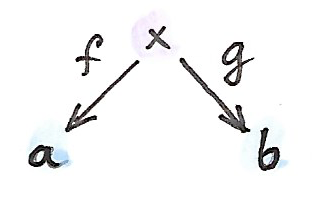
\includegraphics[width=1.46875in]{images/span.png}\\
You might recall that we used spans in the definition of a categorical
product. Here, we want to look at spans as 1-cells in a bicategory. The
first step is to define a composition of spans. Suppose that we have an
adjoining span:

\begin{verbatim}
f':: y -> b g':: y -> c
\end{verbatim}

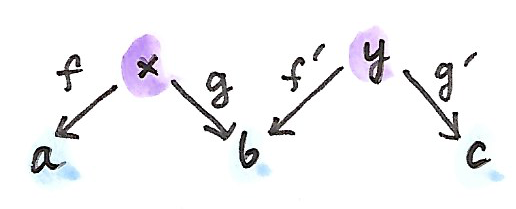
\includegraphics[width=2.26042in]{images/compspan.png}\\
The composition would be a third span, with some apex \code{z}. The
most natural choice for it is the pullback of \code{g} along
\code{f\'}. Remember that a pullback is the object \code{z}
together with two morphisms:

\begin{verbatim}
h :: z -> x h':: z -> y
\end{verbatim}

such that:

\begin{verbatim}
g ∘ h = f' ∘ h'
\end{verbatim}

which is universal among all such objects.

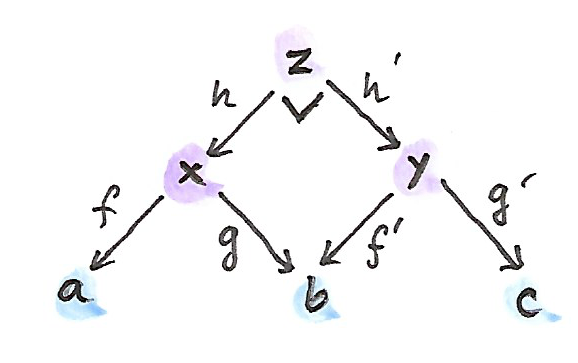
\includegraphics[width=2.42708in]{images/pullspan.png}\\
For now, let's concentrate on spans over the category of sets. In that
case, the pullback is just a set of pairs \code{(p,\ q)} from the
cartesian product \code{x\ ×\ y} such that:

\begin{verbatim}
g p = f' q
\end{verbatim}

A morphism between two spans that share the same endpoints is defined as
a morphism \code{h} between their apices, such that the appropriate
triangles commute.

\hypertarget{attachment_9111}{}
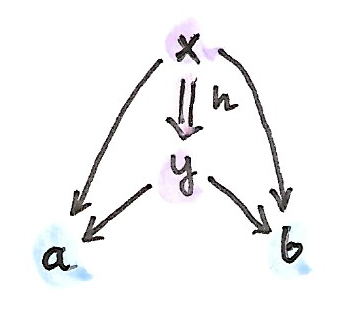
\includegraphics[width=1.70833in]{images/morphspan.png}

A 2-cell in \textbf{Span}.

To summarize, in the bicategory \textbf{Span}: 0-cells are sets, 1-cells
are spans, 2-cells are span morphisms. An identity 1-cell is a
degenerate span in which all three objects are the same, and the two
morphisms are identities.

We've seen another example of a bicategory before: the bicategory
\textbf{Prof} of
\href{https://bartoszmilewski.com/2017/03/29/ends-and-coends/}{profunctors},
where 0-cells are categories, 1-cells are profunctors, and 2-cells are
natural transformations. The composition of profunctors was given by a
coend.

\section{Monads}\label{monads}

By now you should be pretty familiar with the definition of a monad as a
monoid in the category of endofunctors. Let's revisit this definition
with the new understanding that the category of endofunctors is just one
small hom-category of endo-1-cells in the bicategory \textbf{Cat}. We
know it's a monoidal category: the tensor product comes from the
composition of endofunctors. A monoid is defined as an object in a
monoidal category --- here it will be an endofunctor \code{T} ---
together with two morphisms. Morphisms between endofunctors are natural
transformations. One morphism maps the monoidal unit --- the identity
endofunctor --- to \code{T}:

\begin{verbatim}
η :: I -> T
\end{verbatim}

The second morphism maps the tensor product of \code{T\ ⊗\ T} to
\code{T}. The tensor product is given by endofunctor composition, so
we get:

\begin{verbatim}
μ :: T ∘ T -> T
\end{verbatim}

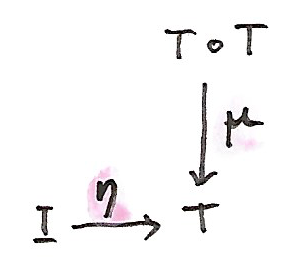
\includegraphics[width=1.35417in]{images/monad.png}\\
We recognize these as the two operations defining a monad (they are
called \code{return} and \code{join} in Haskell), and we know that
monoid laws turn to monad laws.

Now let's remove all mention of endofunctors from this definition. We
start with a bicategory \code{C} and pick a 0-cell \code{a} in it.
As we've seen earlier, the hom-category \code{C(a,\ a)} is a monoidal
category. We can therefore define a monoid in \code{C(a,\ a)} by
picking a 1-cell, \code{T}, and two 2-cells:

\begin{verbatim}
η :: I -> T μ :: T ∘ T -> T
\end{verbatim}

satisfying the monoid laws. We call \emph{this} a monad.

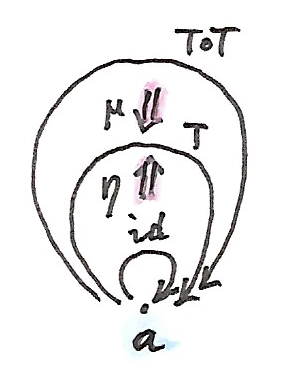
\includegraphics[width=1.39583in]{images/bimonad.png}\\
That's a much more general definition of a monad using only 0-cells,
1-cells, and 2-cells. It reduces to the usual monad when applied to the
bicategory \textbf{Cat}. But let's see what happens in other
bicategories.

Let's construct a monad in \textbf{Span}. We pick a 0-cell, which is a
set that, for reasons that will become clear soon, I will call
\code{Ob}. Next, we pick an endo-1-cell: a span from \code{Ob} back
to \code{Ob}. It has a set at the apex, which I will call \code{Ar},
equipped with two functions:

\begin{verbatim}
dom :: Ar -> Ob cod :: Ar -> Ob
\end{verbatim}

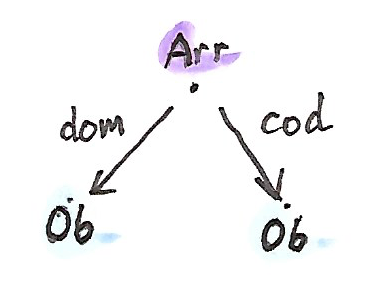
\includegraphics[width=1.91667in]{images/spanmonad.png}\\
Let's call the elements of the set \code{Ar} ``arrows.'' If I also
tell you to call the elements of \code{Ob} ``objects,'' you might get
a hint where this is leading to. The two functions \code{dom} and
\code{cod} assign the domain and the codomain to an ``arrow.''

To make our span into a monad, we need two 2-cells, \code{η} and
\code{μ}. The monoidal unit, in this case, is the trivial span from
\code{Ob} to \code{Ob} with the apex at \code{Ob} and two identity
functions. The 2-cell \code{η} is a function between the apices
\code{Ob} and \code{Arr}. In other words, \code{η} assigns an
``arrow'' to every ``object.'' A 2-cell in \textbf{Span} must satisfy
commutation conditions --- in this case:

\begin{verbatim}
dom ∘ η = id cod ∘ η = id
\end{verbatim}

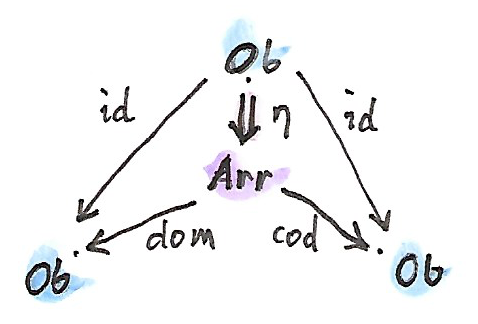
\includegraphics[width=2.27083in]{images/spanunit.png}\\
In components, this becomes:

\begin{verbatim}
dom (η ob) = ob = cod (η ob)
\end{verbatim}

where \code{ob} is an ``object'' in \code{Ob}. In other words,
\code{η} assigns to every ``object'' and ``arrow'' whose domain and
codomain are that ``object.'' We'll call this special ``arrow'' the
``identity arrow.''

The second 2-cell \code{μ} acts on the composition of the span
\code{Ar} with itself. The composition is defined as a pullback, so
its elements are pairs of elements from \code{Ar} --- pairs of
``arrows'' \code{(a1,\ a2)}. The pullback condition is:

\begin{verbatim}
cod a1 = dom a2
\end{verbatim}

We say that \code{a1} and \code{a1} are ``composable,'' because the
domain of one is the codomain of the other.\\
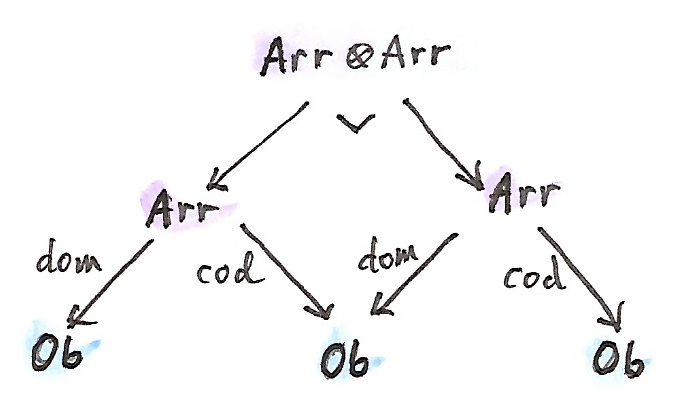
\includegraphics[width=2.75000in]{images/spanmul.png}

The 2-cell \code{μ} is a function that maps a pair of composable
arrows \code{(a1,\ a2)} to a single arrow \code{a3} from
\code{Ar}. In other words \code{μ} defines composition of arrows.

It's easy to check that monad laws correspond to identity and
associativity laws for arrows. We have just defined a category (a small
category, mind you, in which objects and arrows form sets).

So, all told, a category is just a monad in the bicategory of spans.

What is amazing about this result is that it puts categories on the same
footing as other algebraic structures like monads and monoids. There is
nothing special about being a category. It's just two sets and four
functions. In fact we don't even need a separate set for objects,
because objects can be identified with identity arrows (they are in
one-to-one correspondence). So it's really just a set and a few
functions. Considering the pivotal role that category theory plays in
all of mathematics, this is a very humbling realization.

\section{Challenges}\label{challenges}

\begin{enumerate}
\tightlist
\item
  Derive unit and associativity laws for the tensor product defined as
  composition of endo-1-cells in a bicategory.
\item
  Check that monad laws for a monad in \textbf{Span} correspond to
  identity and associativity laws in the resulting category.
\item
  Show that a monad in \textbf{Prof} is an identity-on-objects functor.
\item
  What's a monad algebra for a monad in \textbf{Span}?
\end{enumerate}

\section{Bibliography}\label{bibliography}
